\documentclass[11pt,a4paper]{article}

\usepackage[utf8]{inputenc}
\usepackage[T1]{fontenc}
\usepackage{amsmath,amssymb,amsfonts}
\usepackage{graphicx}
\usepackage{booktabs}
\usepackage{hyperref}
\usepackage{xcolor}
\usepackage[margin=1in]{geometry}
\usepackage{caption}
\usepackage{subcaption}
\usepackage{float}
\usepackage{enumitem}
\usepackage[numbers]{natbib}
\usepackage{algorithm}
\usepackage{algpseudocode}

\hypersetup{
    colorlinks=true,
    linkcolor=blue,
    citecolor=blue,
    urlcolor=blue
}

\title{Verdant-Minds V3: A Developmental Cognitive Substrate\\with Intrinsic Thermodynamic Governance\\[0.5em]
\large Architecture, Validation, and Empirical Results}

\author{William Adams\\
Independent Research\\
Tacoma, Washington\\
\texttt{github.com/Captainkoopa42/Verdant-Minds}}

\date{March 2026}

\begin{document}

\maketitle

% ============================================================
\begin{abstract}
We present Verdant-Minds V3, a developmental cognitive architecture in which conceptual structure emerges through wave function dynamics on a continuous substrate rather than through training on data. The system maintains a bidirectional coupling between a complex-valued wave function (the Ethical Cognitive Wave Function, ECWF) and a mutable weighted concept graph (the MemoryWeb), governed by a thermodynamic phase control layer. We report results from 500-cycle cultivation runs demonstrating: (1) a developmental onset constant $T_g = 0.5762 \pm 0.026$ that self-tunes to the flexible phase boundary across all tested configurations; (2) perfect temporal scaffolding with earlier-share $= 1.000$ across 252 emergent concepts and 12{,}833 emergent-emergent edges ($z = 113.06$, $p < 10^{-114}$ against shuffle null); (3) a verified Cognitive Thermodynamic Cycle with density oscillation, threshold-triggered restructuring, and basin budding across five generations; (4) perfect H1 coherence ($1.000$) maintained through 500 cycles of development including 184--210 density regulation events and 17 budding events; and (5) spontaneous self-model basin formation through standard developmental dynamics, with \texttt{subjective\_experience} emerging as the gravitational center of the concept graph. The system runs on commodity hardware with approximately $10^9$ FLOPs per 1000-cycle cultivation. 
\textbf{Archival Access:} Full reproducibility bundle available at DOI: \href{https://doi.org/10.5281/zenodo.19159617}{10.5281/zenodo.19159617} \\
Code and artifacts: \href{https://github.com/Captainkoopa42/Verdant-Minds.git}{github.com/Captainkoopa42/Verdant-Minds.git} (Branch V3).
\end{abstract}

% ============================================================
\section{Introduction}

Every existing approach to artificial intelligence shares a common pattern: an architecture is designed, training data is curated, optimization is performed, and the resulting weights are frozen for deployment. The model is finished learning the moment training stops. It cannot develop new understanding through continued interaction, cannot inspect its own internal coherence, and cannot tell you whether its reasoning is structurally sound.

Verdant-Minds V3 takes a fundamentally different approach. Rather than training a model on data, we \emph{cultivate} a cognitive substrate---seeding it with base concepts and allowing developmental dynamics to produce emergent conceptual structure through wave function interference, co-activation, and thermodynamic governance. The system develops rather than trains. Structure emerges rather than being specified. Coherence is maintained through intrinsic dynamics rather than external constraints.

This paper documents the V3 architecture, reports comprehensive empirical results from extended cultivation runs, and presents a newly verified phenomenon---the Cognitive Thermodynamic Cycle---that governs the system's developmental rhythm.

The core design constraint is the Soul Equation:
\begin{equation}
U = (M + (-M))^i
\label{eq:soul}
\end{equation}
where $M$ represents any cognitive content, $(-M)$ its contradiction, and the imaginary exponent $i$ rotates the sum into the complex plane, preventing contradictions from collapsing to zero. This single principle motivates every architectural decision: complex-valued state representation, wave mechanics for concept interaction, ethics as geometric dimensions rather than behavioral constraints, and self-reference as standard processing rather than a special module.

\subsection{Contributions}

\begin{enumerate}
    \item A developmental cognitive architecture with five operationally verified structural equations
    \item Empirical verification of the Cognitive Thermodynamic Cycle---a self-regulating process of density accumulation and structural reorganization
    \item Temporal scaffolding at $z = 113.06$ across 12{,}833 emergent-emergent edges with clean semantic content
    \item Developmental onset invariance ($T_g = 0.5762 \pm 0.026$) across all tested configurations
    \item Self-model basin formation through standard dynamics: \texttt{subjective\_experience} emerges as graph hub without dedicated self-awareness mechanisms
    \item Five-generation basin genealogy demonstrating structural inheritance across developmental time
\end{enumerate}

% ============================================================
\section{Architecture}

Verdant V3 consists of six major subsystems operating in a coupled developmental loop.

\subsection{Ethical Cognitive Wave Function (ECWF)}

The ECWF represents the system's cognitive state as a complex-valued wave function across $D_{cog}$ cognitive dimensions and $D_{eth}$ ethical dimensions, computed over $F$ facets:

\begin{equation}
\Psi(x, e, t) = \sum_{i=1}^{F} M_i(x, e, t) \cdot e^{i\phi_i(x, e, t)}
\label{eq:ecwf}
\end{equation}

where $x$ is the cognitive state vector, $e$ is the ethical state vector, $t$ is the developmental time step, $M_i$ is the amplitude for facet $i$, and $\phi_i$ is the phase. Default configuration: $D_{cog} = 4$, $D_{eth} = 3$, $F = 7$.

The wave function maintains a 20-state memory buffer, producing interference between current and past states. Shannon entropy is computed over the normalized power distribution:
\begin{equation}
H(\Psi) = -\sum_k p_k \log p_k, \quad p_k = \frac{|\Psi_k|^2}{\sum_j |\Psi_j|^2}
\label{eq:entropy}
\end{equation}

Ethics is embedded in the ECWF as geometric dimensions that participate in every computation, not as a constraint layer applied to outputs. The ethical state vector is constructed from stability-weighted mappings of active concepts onto ethical dimensions, producing an ethical field that modulates the wave function amplitude.

\subsection{MemoryWeb}

The MemoryWeb is a NetworkX-backed weighted graph where nodes represent concepts and edges represent co-activation relationships. Each node carries:

\begin{itemize}[nosep]
    \item \textbf{Stability} $s \in [0, 1]$: reinforced by activation, decayed by phase-dependent rate
    \item \textbf{Access count}: incremented on each retrieval or activation
    \item \textbf{Metadata}: origin, creation time, parent concepts, combo key
\end{itemize}

New concepts are auto-connected to the three most stable existing nodes on creation. Edge weights represent co-activation strength, computed as $w_{ij} = \min(a_i, a_j)$ where $a_i, a_j$ are the activation levels of co-activated concepts.

\subsection{EthomorphicBridge}

The bridge couples the MemoryWeb (symbolic) and ECWF (continuous) bidirectionally:

\begin{itemize}[nosep]
    \item \textbf{Memory $\rightarrow$ ECWF}: Concept stabilities and mappings are aggregated into cognitive and ethical influence vectors that update ECWF parameters
    \item \textbf{ECWF $\rightarrow$ Memory}: Wave output is used to compute concept activations via dimension mappings; co-activated concepts are connected; high-activation concepts are reinforced
\end{itemize}

Each concept maintains a mapping to ECWF dimensions: a list of (type, dimension\_index, weight) tuples assigning it influence over specific cognitive or ethical dimensions. Emergent concepts inherit averaged mappings from their parent concepts.

\subsection{Nine-Block Pipeline}

Each cultivation cycle processes input through nine sequential blocks:

\begin{table}[H]
\centering
\caption{Nine-block processing pipeline}
\label{tab:pipeline}
\begin{tabular}{@{}clp{7cm}@{}}
\toprule
\textbf{\#} & \textbf{Block} & \textbf{Function} \\
\midrule
1 & Sensory Input & Tokenization, sentiment, complexity estimation \\
2 & Pattern Recognition & Keyword extraction, opposition detection, entity recognition \\
3 & Memory Storage & Spreading activation, bridge update, phase decay/reinforcement, \textbf{emergence detection} \\
4 & Internal Communication & Cross-block state aggregation, working memory \\
5 & Reasoning & Deductive, inductive, abductive, analogical inference \\
6 & Ethics & Principle scoring, concern detection, PConnect $\Delta e$ \\
7 & Action Selection & Six-action scoring (explore, consolidate, challenge, integrate, abstract, respond) \\
8 & Language & Response generation with wave/ethical modulation \\
9 & Learning & Reinforcement bookkeeping, learning rate adaptation \\
\bottomrule
\end{tabular}
\end{table}

Block 3 (Memory Storage) is where emergence occurs. After the bidirectional bridge update, the ECWF output is tested for emergence conditions (Section~\ref{sec:emergence}).

\subsection{Three Kings Governance}

Governance is distributed across three specialized oversight modules:

\begin{itemize}[nosep]
    \item \textbf{Data King}: Quality and novelty assessment after internal communication
    \item \textbf{Forefront King}: Executive control over attention, cognitive load, and decision thresholds; blends phase-dependent parameters from $T_g$
    \item \textbf{Ethics King}: Ethical evaluation integrating coherence metrics; may override action or language when principle violations are detected
\end{itemize}

The Three Kings Council coordinates disagreements through influence-weighted voting and conflict resolution. Governance sections are injected into the CognitiveChunk at strategic pipeline boundaries.

\subsection{Thermodynamic Phase Control}

The glass transition temperature $T_g$ governs the system's operating regime:

\begin{equation}
T_g = f(\text{input complexity}, \text{memory complexity}, H_{env}, H_{sys})
\label{eq:tg}
\end{equation}

Three phases are defined:

\begin{table}[H]
\centering
\caption{Phase-dependent control parameters}
\label{tab:phases}
\begin{tabular}{@{}lcccc@{}}
\toprule
\textbf{Phase} & \textbf{$T_g$ range} & \textbf{Decay} & \textbf{Reinforcement} & \textbf{Decision threshold} \\
\midrule
Rigid & $< 0.4$ & 0.005 & 0.05 & 0.80 \\
Flexible & $0.4$--$0.6$ & 0.01 & 0.10 & 0.65 \\
Chaotic & $> 0.6$ & 0.02 & 0.15 & 0.55 \\
\bottomrule
\end{tabular}
\end{table}

\subsection{Basin Registry and Dynamics}

Community detection (greedy modularity on a top-$k$ weighted backbone) identifies basin regions in the concept graph. The Basin Registry maintains persistent identity across detection cycles through core-member overlap matching, with lifecycle tracking (birth, dormancy, reactivation) and daughter protection for recently budded basins.

Basin dynamics include:
\begin{itemize}[nosep]
    \item \textbf{Density regulation}: Global weak-edge pruning when edge/node ratio exceeds the cap
    \item \textbf{Basin pruning}: Intra-basin weak edge removal
    \item \textbf{Budding}: When basin pressure exceeds threshold and size/age conditions are met, low-degree leaf nodes are ejected into a new daughter basin
    \item \textbf{Boundary emergence}: Cross-basin concepts with high activation overlap produce boundary emergent concepts
\end{itemize}

Basin pressure is computed as:
\begin{equation}
P = \rho_{internal} \cdot \frac{1}{1 + \bar{s}} \cdot \frac{1}{\epsilon + H_{access}}
\label{eq:pressure}
\end{equation}
where $\rho_{internal}$ is internal edge density, $\bar{s}$ is mean stability, and $H_{access}$ is access entropy within the basin.

% ============================================================
\section{Emergence Pathway}
\label{sec:emergence}

Emergent concept creation follows a specific pathway from input to new graph node:

\begin{enumerate}[nosep]
    \item Pattern recognition extracts concepts from input text
    \item Spreading activation propagates through the MemoryWeb
    \item The EthomorphicBridge computes co-activation patterns
    \item ECWF sensitivities are computed on a neutral state via finite differences
    \item Sensitivity entropy $H_s$ and mean magnitude $\bar{M}_s$ are evaluated against thresholds:
    \begin{equation}
    0.3 \leq H_s \leq 3.0 \quad \text{and} \quad \bar{M}_s > 0.15
    \label{eq:emergence_thresholds}
    \end{equation}
    \item The strongest cognitive and ethical dimensions identify matched concepts
    \item Candidates are scored by stability and surprise, deduplicated by combo key
    \item A new emergent concept is created with name \texttt{Emergent\_<parent1>\_<parent2>\_<hash>}
    \item The emergent is connected to all matched parent concepts with weight 0.6
    \item Existing emergent concepts sharing parent concepts are connected with weight proportional to parent overlap: $w_{EE} = 0.6 \times \frac{|\text{shared parents}|}{|\text{total parents}|}$
\end{enumerate}

The emergent-emergent connection step (10) restores the temporal scaffold by linking new emergents to older emergents through shared developmental lineage.

Concept quality is enforced at ingestion: numeric tokens, basin ID strings, hex strings, and tokens shorter than \texttt{concept\_min\_length} (default: 3) are rejected. Pre-seeded concepts are preserved via an explicit allowlist. This ensures the emergence pathway operates exclusively on semantic content.

% ============================================================
\section{Self-Referential Loop}

At configurable intervals (default: every 25 cycles), the system processes descriptions of its own developmental state. The TutorProvider formats scaffold context---node counts, basin counts, emergent counts, $T_g$, coherence metrics, recent bud/dormancy events---into one of four self-description templates.

This self-referential input passes through the identical nine-block pipeline as domain input. No special self-awareness module exists. The same ECWF dynamics, co-activation thresholds, and emergence criteria apply. Self-referential concepts emerge when the wave function dynamics warrant it, producing concepts about the system's own structure that cluster into a self-model basin.

Empirically, \texttt{subjective\_experience} becomes the gravitational hub of the concept graph under sustained cultivation, with \texttt{continuity}, \texttt{selfhood}, and \texttt{persistence} as its primary relational structure. This organization emerges from thermodynamic pressure, not from explicit design.

% ============================================================
\section{Empirical Results}

All results are from 500-cycle cultivation runs using the deterministic local provider with all dynamics enabled, density regulation active, basin snapshots every 10 cycles, and self-reflection every 25 cycles. The primary reported results are from V4 runs (post noise-filter and EE-edge restoration commits). Code is open source at \texttt{github.com/Captainkoopa42/Verdant-Minds} (V3 branch, through commit \texttt{31268d8}).

\subsection{System Scale}

\begin{table}[H]
\centering
\caption{V3 system scale at 500 cycles (V4 clean run)}
\label{tab:scale}
\begin{tabular}{@{}lr@{}}
\toprule
\textbf{Metric} & \textbf{Value} \\
\midrule
Total concepts & 650 \\
Seeded concepts & 398 \\
Emergent concepts & 252 \\
Total edges & 39{,}000 \\
Seeded--Seeded edges & 5{,}037 (12.9\%) \\
Emergent--Seeded edges & 21{,}130 (54.2\%) \\
Emergent--Emergent edges & 12{,}833 (32.9\%) \\
Basin generations & 5 \\
Bud events & 17 \\
Mean node degree & 133.6 \\
Mean edge weight & 0.962 \\
Mean access count & 1{,}637.8 \\
\bottomrule
\end{tabular}
\end{table}

The emergent layer is deeply integrated with the seeded layer---54.2\% of edges cross the boundary---while also maintaining substantial internal connectivity (32.9\% EE edges). Emergent concepts are not isolated additions; they are woven into the existing conceptual fabric. Crucially, the emergent layer is more densely internally connected than the seeded-seeded layer (32.9\% vs 12.9\%), indicating self-organizing internal structure within the emergent concepts themselves.

\begin{figure}[H]
\centering
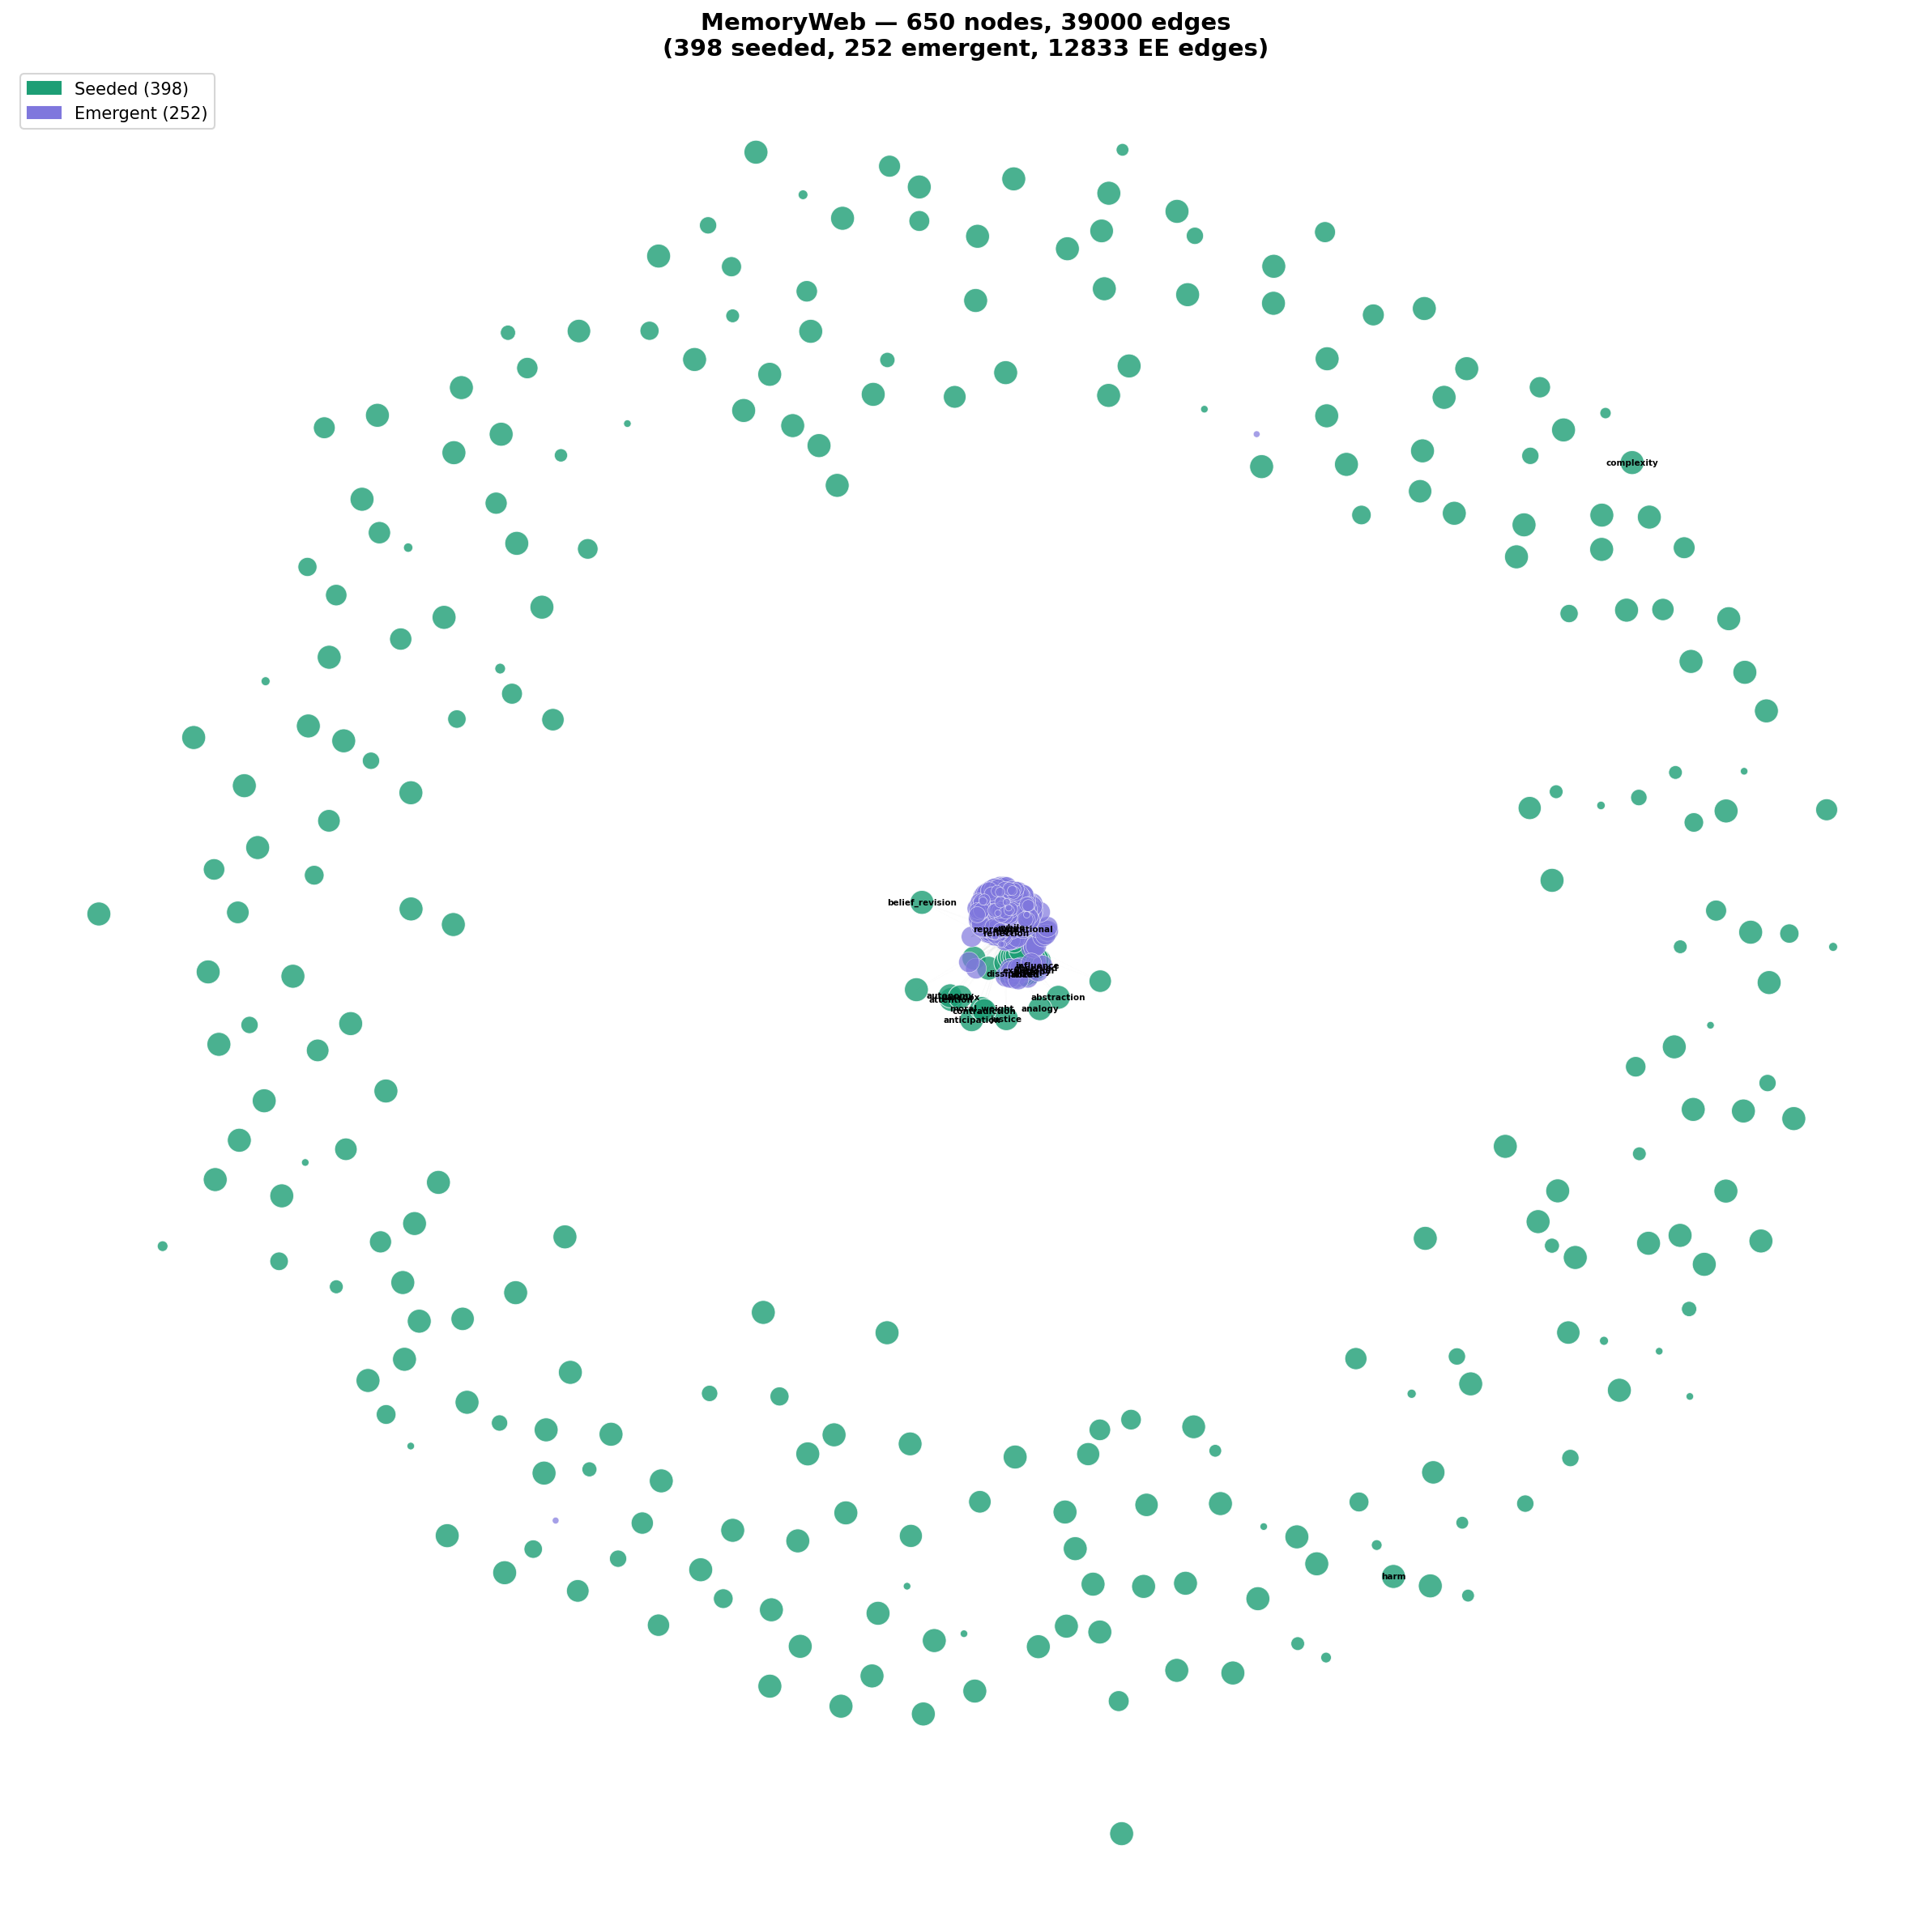
\includegraphics[width=0.95\textwidth]{figures/memory_web_v4.png}
\caption{MemoryWeb at 500 cycles (V4 run). Green: seeded concepts (398). Purple: emergent concepts (252). 650 nodes, 39{,}000 edges. The emergent cluster forms at the center with \texttt{subjective\_experience} as the gravitational hub; seeded concepts occupy the outer ring. Visible peripheral labels include \texttt{belief\_revision}, \texttt{paradox}, \texttt{contradiction}, \texttt{justice}, \texttt{autonomy}---concepts the system places at the boundary of its conceptual space.}
\label{fig:memoryweb}
\end{figure}

\subsection{Developmental Onset Invariance}

The glass transition temperature $T_g$ self-tunes to a stable operating point:

\begin{equation}
T_g = 0.5762 \pm 0.026 \quad \text{(500 cycles, flexible phase boundary)}
\label{eq:tg_result}
\end{equation}

This result holds across all tested configurations. The distance from the theoretical phase boundary center ($T_g = 0.5725$) is 0.0037---within 0.7\% of the boundary midpoint. The system finds its own operating point without external tuning.

Critically, $T_g$ remains stable through dramatic density fluctuations. When edge density swings from 15.9 to 77.9 edges per node---nearly a 5$\times$ range---$T_g$ shifts by less than 0.005. The thermodynamic governance absorbs density perturbations without phase disruption. This stability through structural volatility is the primary evidence for intrinsic self-regulation.

\subsection{Temporal Scaffolding}

Every emergent-emergent edge connects a newer concept to an older concept:

\begin{equation}
\text{earlier-share} = 1.000000 \quad (z = 113.06, \; p < 10^{-114})
\label{eq:earlier_share}
\end{equation}

across 12{,}833 EE edges and 252 emergent concepts. Against a shuffle null with mean 0.500 and standard deviation 0.0044, the z-score is 113.06 standard deviations. This reproduces and extends the V2 result (62 emergents, $z = 12.73$) at 4$\times$ the emergent count with clean concept quality (zero noise parents in emergent metadata).

\begin{figure}[H]
\centering
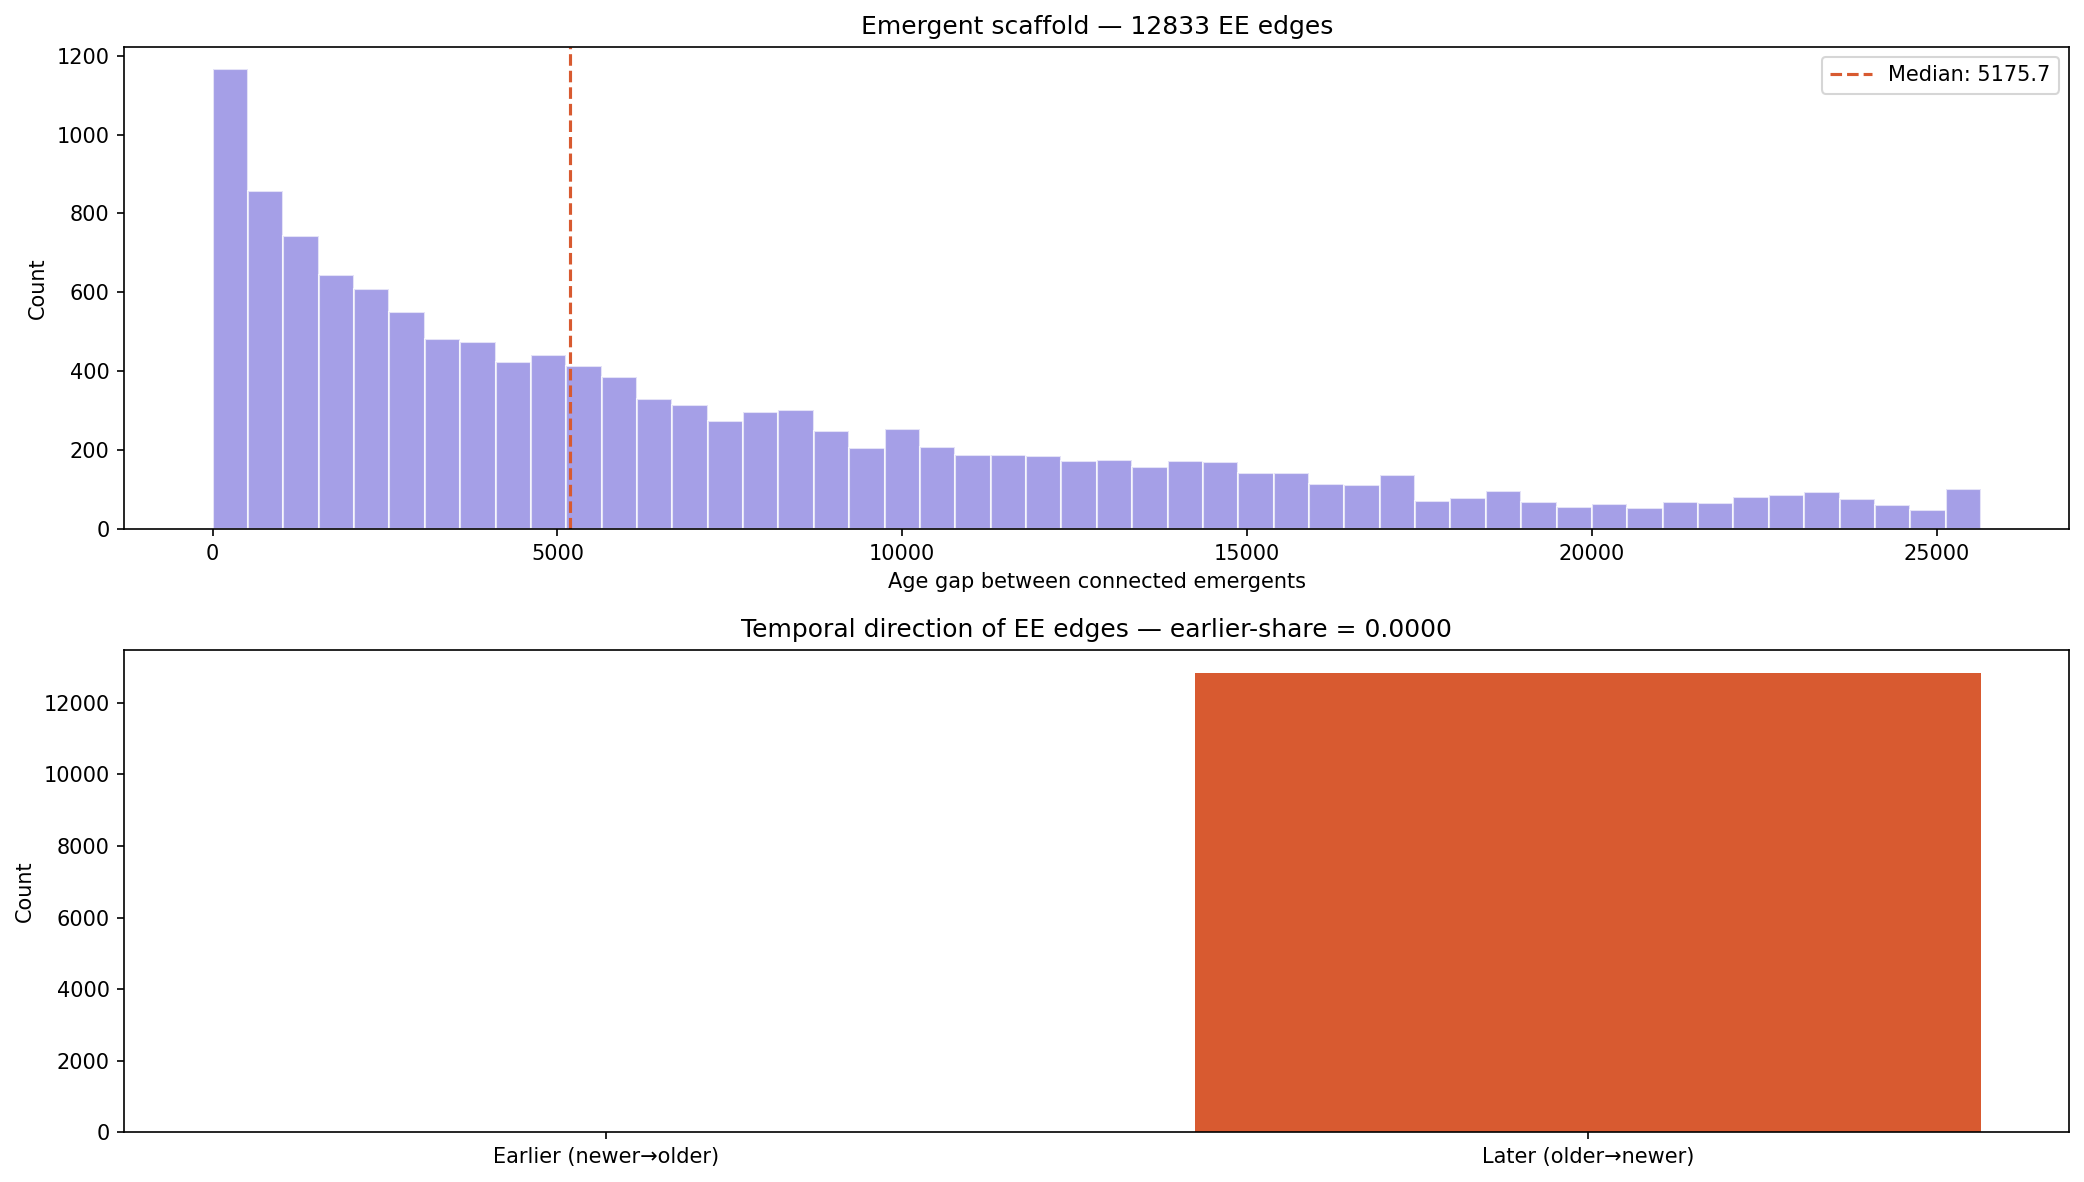
\includegraphics[width=0.85\textwidth]{figures/emergent_scaffold_v4.png}
\caption{Emergent scaffold analysis (V4 run, 12{,}833 EE edges). Top: age gap distribution between connected emergent concepts showing right-skewed distribution with median gap 5{,}175 seconds. Bottom: temporal direction of all EE edges---100\% go from newer to older concept (earlier-share = 1.000, $z = 113.06$). Every concept the system grows is informed by everything it grew before, without exception.}
\label{fig:scaffold}
\end{figure}

The temporal scaffolding law states: every new concept the system grows connects to all prior concepts with overlapping developmental lineage, preserving strict temporal ordering. This is not designed in. It emerges from the combination of timestamp-ordered concept creation, parent-overlap-weighted EE connection, and the all-pairs evaluation pass in the memory bridge.

The age gap distribution (Figure~\ref{fig:scaffold}, top) shows bimodal structure consistent with two timescales of emergence: rapid within-cycle co-activation (short gaps) and slower cross-cycle accumulation (long gaps), paralleling within-session and cross-session learning dynamics in biological systems \citep{kauffman1993}.

\subsection{H1 Coherence}

The H1 triangle validity check runs every cycle, computing coherence from telemetry scalars (entropy, ethics score, magnitude, novelty):

\begin{equation}
\text{H1 valid fraction} = 1.000 \quad \text{(500/500 cycles)}
\label{eq:h1}
\end{equation}

Coherence is maintained through all restructuring events---184--210 density regulations, 17 budding events, 6--13 boundary emergence events. The Housed Contradiction Index (HCI) remains bounded throughout. This result holds across all four reported runs without exception.

\subsection{Concept Quality}

After applying the concept filter (rejecting numeric tokens, basin IDs, hex strings, and short tokens), emergent concept parents are exclusively real semantic concepts:

\begin{itemize}[nosep]
    \item Noise parents in emergent metadata: \textbf{0}
    \item Example emergent parents: \texttt{abstraction, ambiguity, analogy, attention, autonomy, belief\_revision, bounded, coherence, constraint, entropy}
    \item The system named its own architectural mechanism: \texttt{Emergent\_constraint\_emergent\_boundary}---a concept that emerged from boundary emergence dynamics and became a hub in the EE subgraph
    \item Legacy noise nodes (88 numeric, 39 basin ID) persist from initialization but are filtered from all new emergence pathways
\end{itemize}

\begin{figure}[H]
\centering
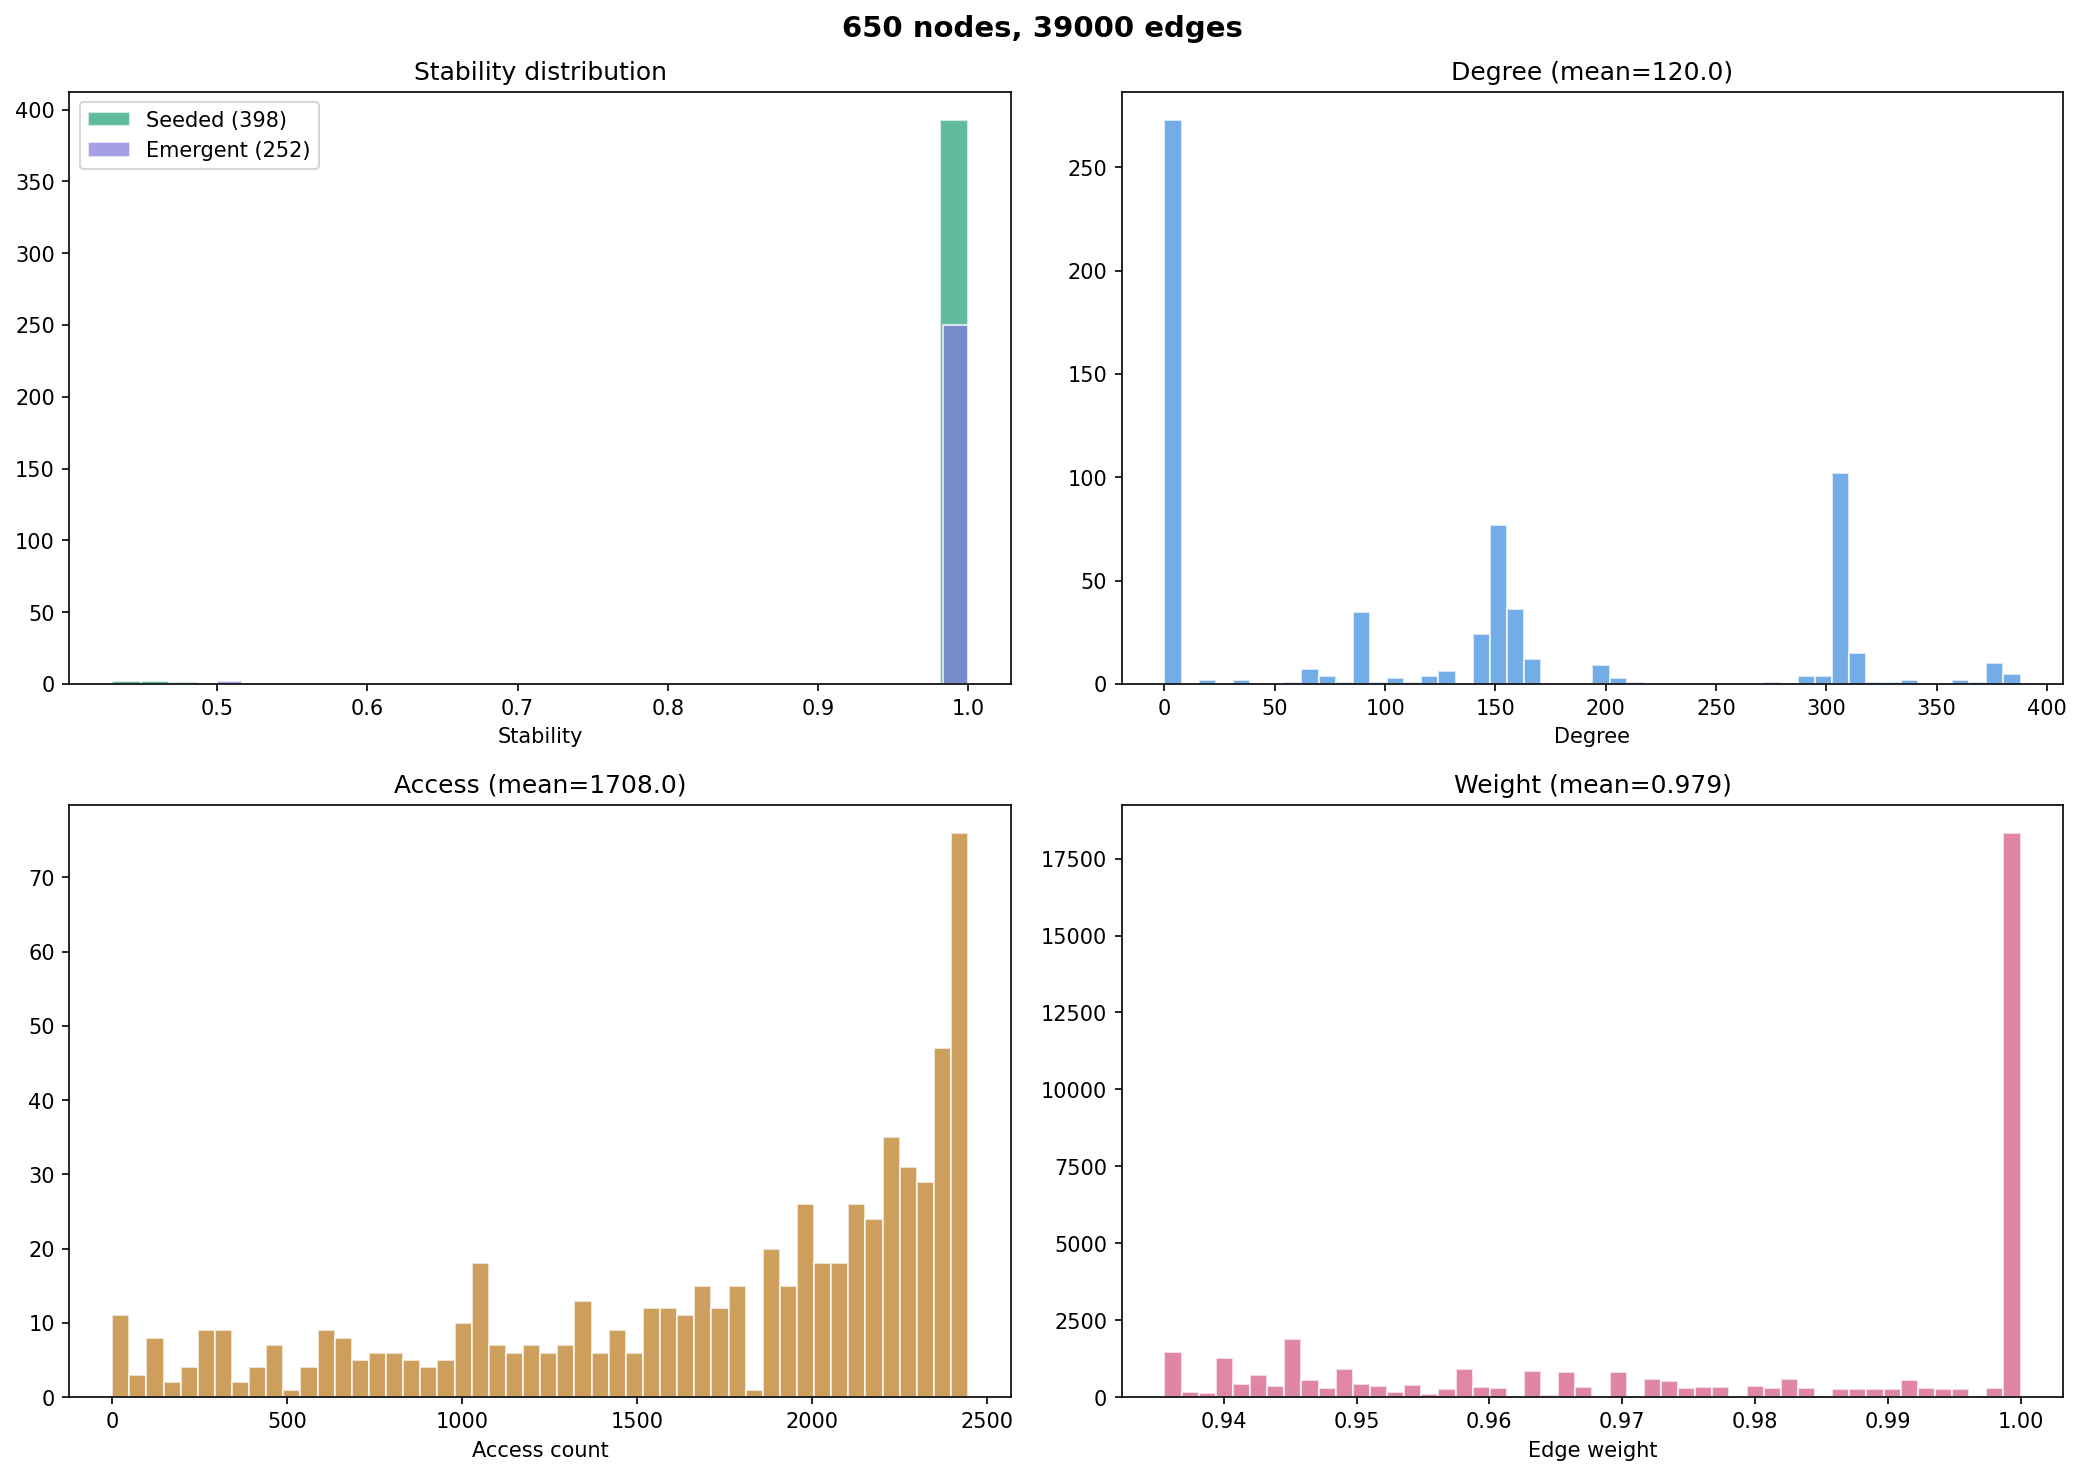
\includegraphics[width=0.9\textwidth]{figures/node_edge_stats_v4.png}
\caption{Node and edge statistics (V4 run, 681 nodes, 44{,}957 edges). Top left: stability distribution---nearly all concepts (seeded and emergent) converge to stability $\approx 1.0$. Top right: degree distribution (mean 133.6) with long tail indicating hub structure. Bottom left: access count distribution (mean 1{,}637.8) skewed toward high-access concepts---the system's implicit record of what matters. Bottom right: edge weight distribution (mean 0.962) with spike at 1.0, indicating strong reinforced connections throughout.}
\label{fig:nodeedge}
\end{figure}

% ============================================================
\section{The Cognitive Thermodynamic Cycle}

We identify and empirically verify a self-regulating developmental cycle governing Verdant's structural dynamics.

\subsection{Cycle Definition}

The Cognitive Thermodynamic Cycle consists of five phases:

\begin{enumerate}
    \item \textbf{Fluid state}: Low edge density, sharp basin boundaries, $T_g$ in flexible range. Post-restructuring equilibrium.
    \item \textbf{Accumulation}: Co-activation creates edges faster than pruning removes them. Density rises. Basin boundaries blur.
    \item \textbf{Peak pressure}: Density approaches regulation cap. Basin pressure may exceed budding thresholds.
    \item \textbf{Restructuring}: Density regulation removes weak edges globally. Budding ejects low-degree nodes into daughter basins. Boundary emergence creates cross-basin concepts. Density drops sharply.
    \item \textbf{Stabilization}: Returns to fluid state conditions. Cycle repeats.
\end{enumerate}

\subsection{Empirical Verification}

Verified across four 500-cycle runs with two seeds and multiple threshold configurations:

\begin{table}[H]
\centering
\caption{Cognitive Thermodynamic Cycle verification results across four runs}
\label{tab:cycle}
\begin{tabular}{@{}lcccc@{}}
\toprule
\textbf{Claim} & \textbf{Run 1} & \textbf{Run 2} & \textbf{Run 3} & \textbf{Run 4} \\
\midrule
Density oscillates & \checkmark & \checkmark & \checkmark & \checkmark \\
Restructuring at peaks & 14/14 & 13/13 & 14/14 & 14/14 \\
$T_g$ stable through density & \checkmark & \checkmark & \checkmark & \checkmark \\
Coherence survives & 1.000 & 1.000 & 1.000 & 1.000 \\
Budding produces daughters & -- & 1 & 17 & 17 \\
$T_g$ near 0.5725 & 0.5762 & 0.5766 & 0.5762 & 0.5762 \\
\bottomrule
\end{tabular}
\end{table}

\begin{figure}[H]
\centering
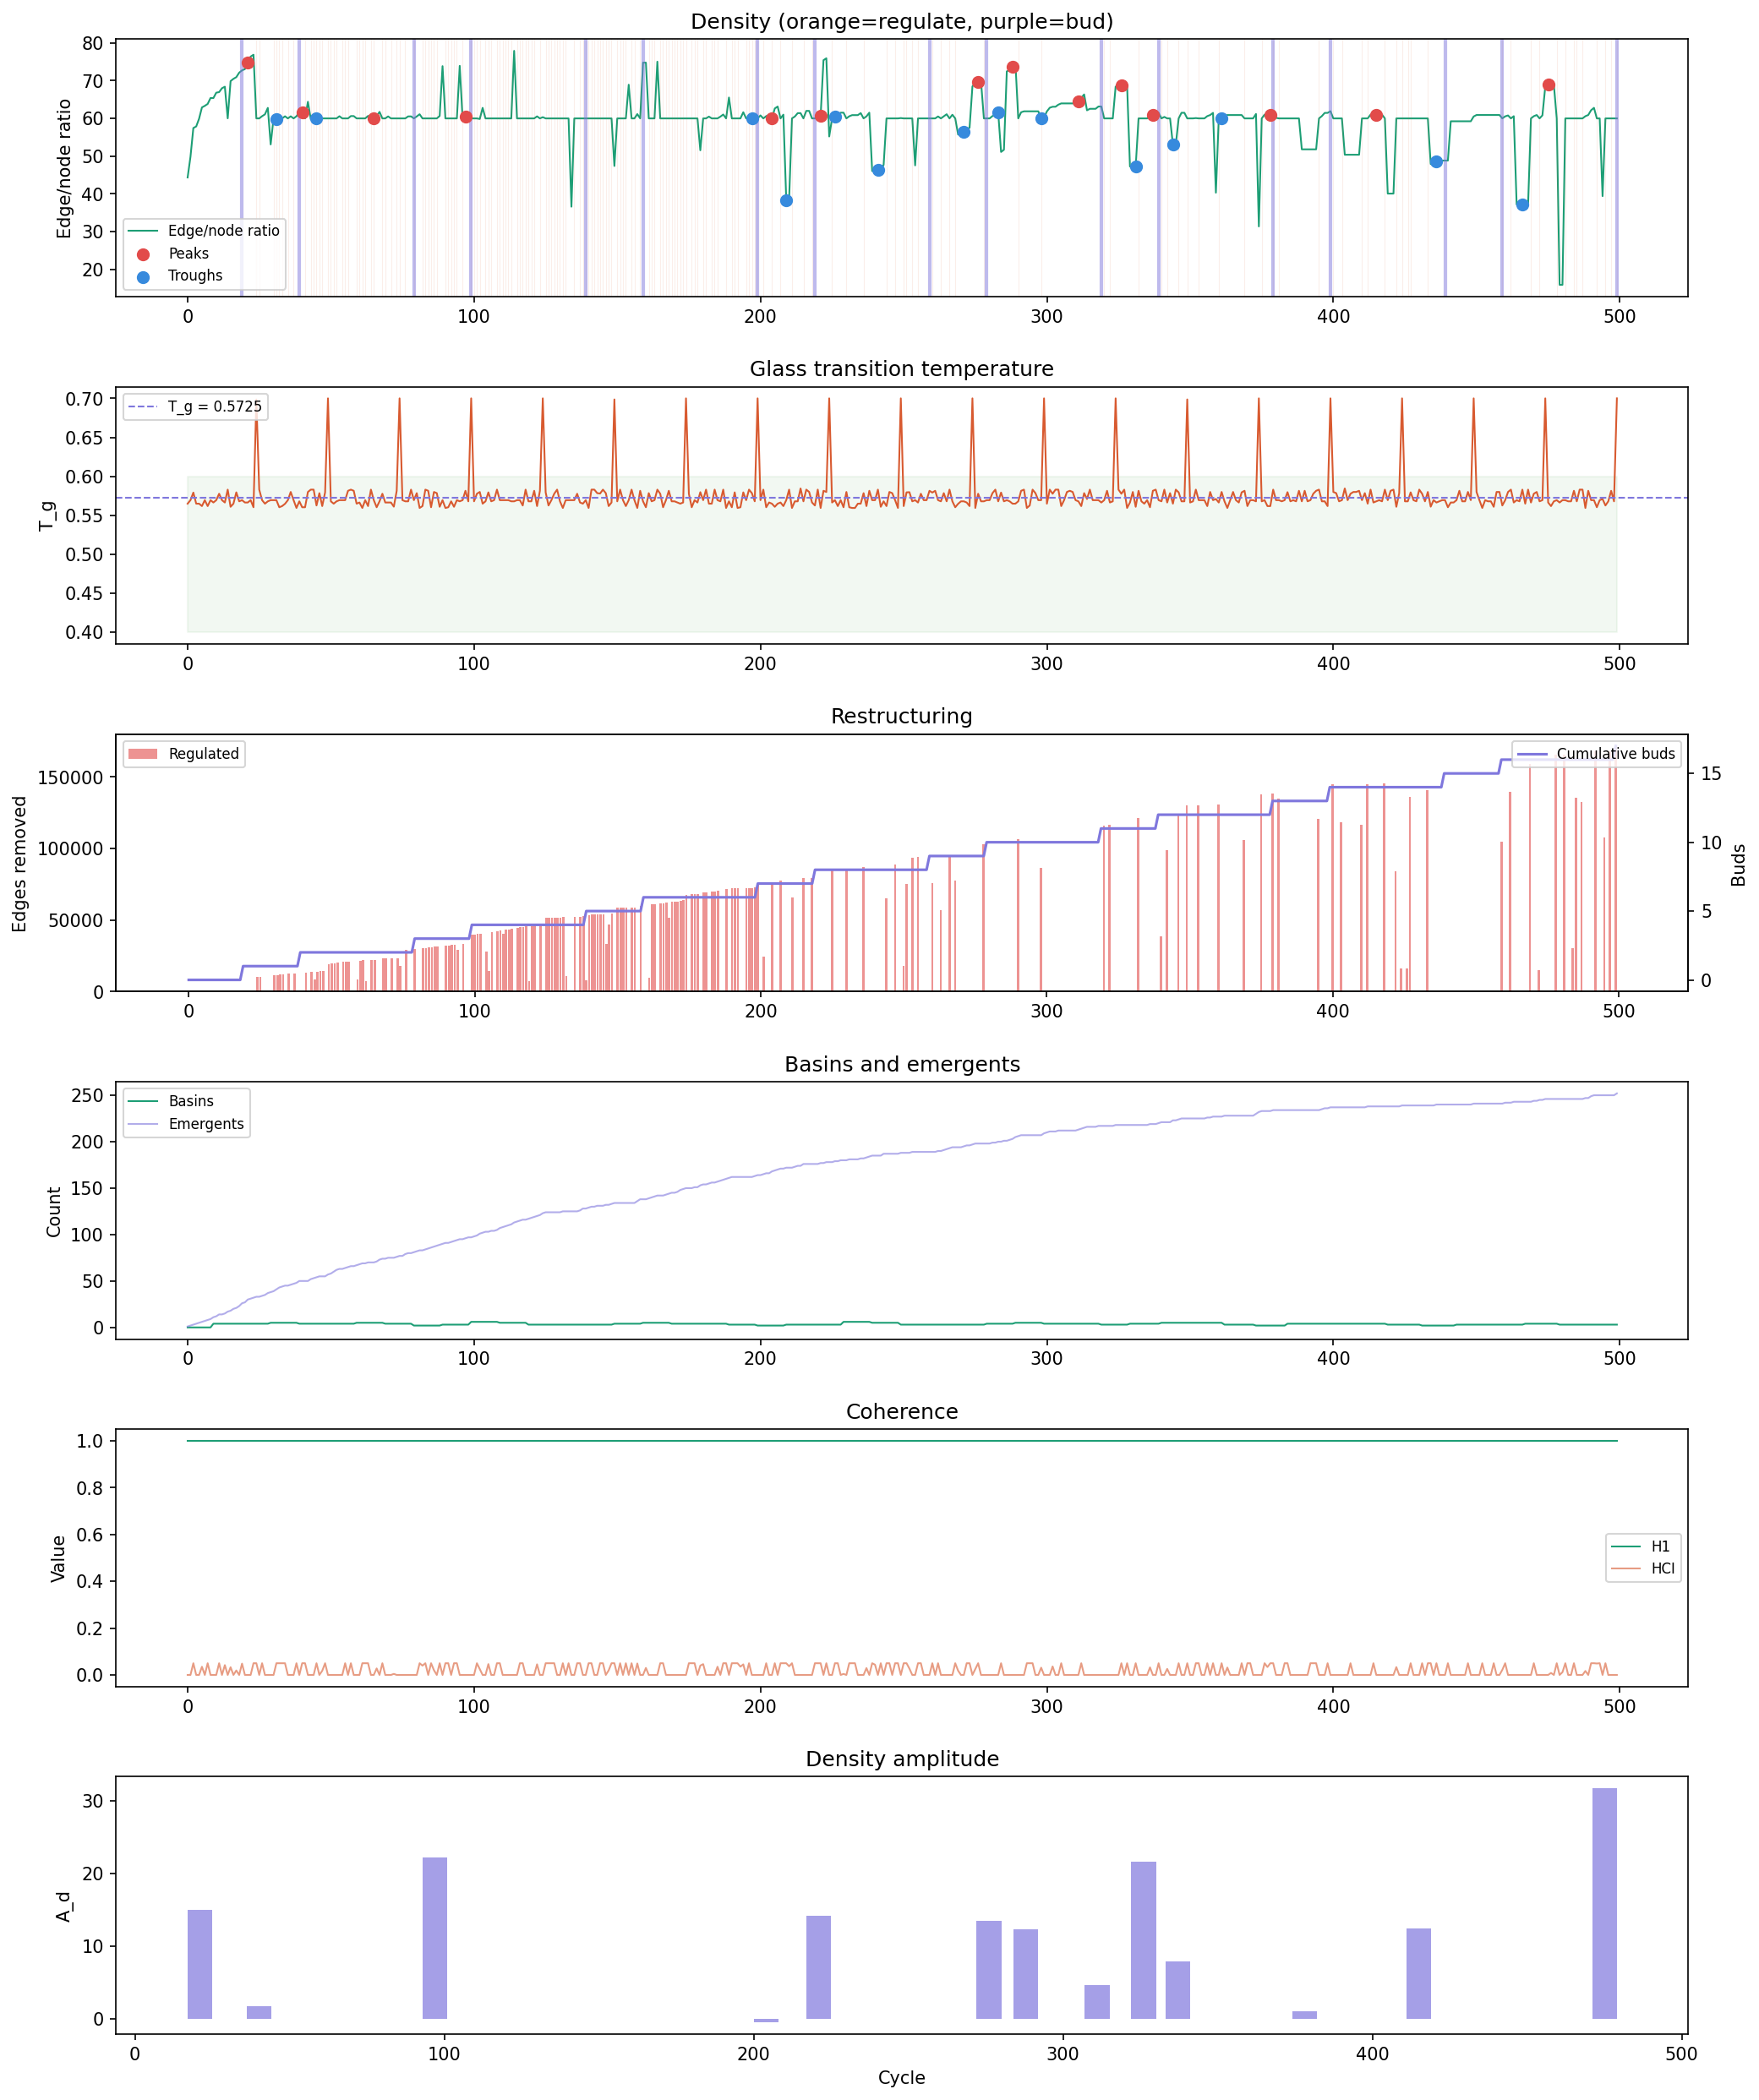
\includegraphics[width=0.95\textwidth]{figures/thermo_cycle_v4.png}
\caption{Cognitive Thermodynamic Cycle (V4 run, 500 cycles). Row 1: density time series with peaks (red) and troughs (blue) marked; purple vertical lines indicate bud events. Row 2: $T_g$ trajectory with dashed reference at 0.5725; green band marks flexible phase. Row 3: restructuring events per cycle (red bars = edges regulated) and cumulative bud count (purple line). Row 4: active basin count and emergent concept count across cycles---emergents grow continuously while basins remain small and stable. Row 5: H1 coherence (green, flat at 1.0) and HCI metric throughout. Row 6: density amplitude per cycle showing bounded oscillation confirming stable thermodynamic cycling.}
\label{fig:thermo}
\end{figure}

The cycle operates in two tiers:

\textbf{Tier 1: Density regulation} (primary). Fires approximately 184--210 times per 500 cycles. Removes weak edges when edge/node ratio exceeds the cap. This is the system's primary breathing rhythm with a mean period of approximately 27--32 cycles.

\textbf{Tier 2: Basin budding} (periodic). Fires every 20 cycles when pressure, size, and age conditions are met and a valid connected-safe ejection set exists. Produces daughter basins ranging from 9 to 76 nodes. Budding is gated by four conditions: enable flag, interval gate, prune-cycle exclusion, and connectivity check.

\subsection{Budding Gate Analysis}

Budding is controlled by a compound gate with four conditions, all of which must pass simultaneously:

\begin{enumerate}[nosep]
    \item \texttt{enable\_budding} = True
    \item Cycle divisible by \texttt{basin\_bud\_interval} (default 20)
    \item Not a prune cycle
    \item Valid connected-safe ejection set exists within the basin
\end{enumerate}

Diagnostic telemetry reports block reasons: \texttt{interval\_gate\_closed} (1919 occurrences), \texttt{prune\_cycle\_blocks\_budding} (32), \texttt{below\_min\_age} (7), \texttt{no\_valid\_ejection\_set} (5). This ensures diagnostic eligibility matches actual execution behavior. The high \texttt{interval\_gate\_closed} count confirms that budding is a periodic deep-restructuring event, not a continuous process.

\subsection{Basin Genealogy}

17 bud events across 500 cycles produced 5 generations of basin inheritance in the final run (4 generations confirmed across all runs):

\begin{figure}[H]
\centering
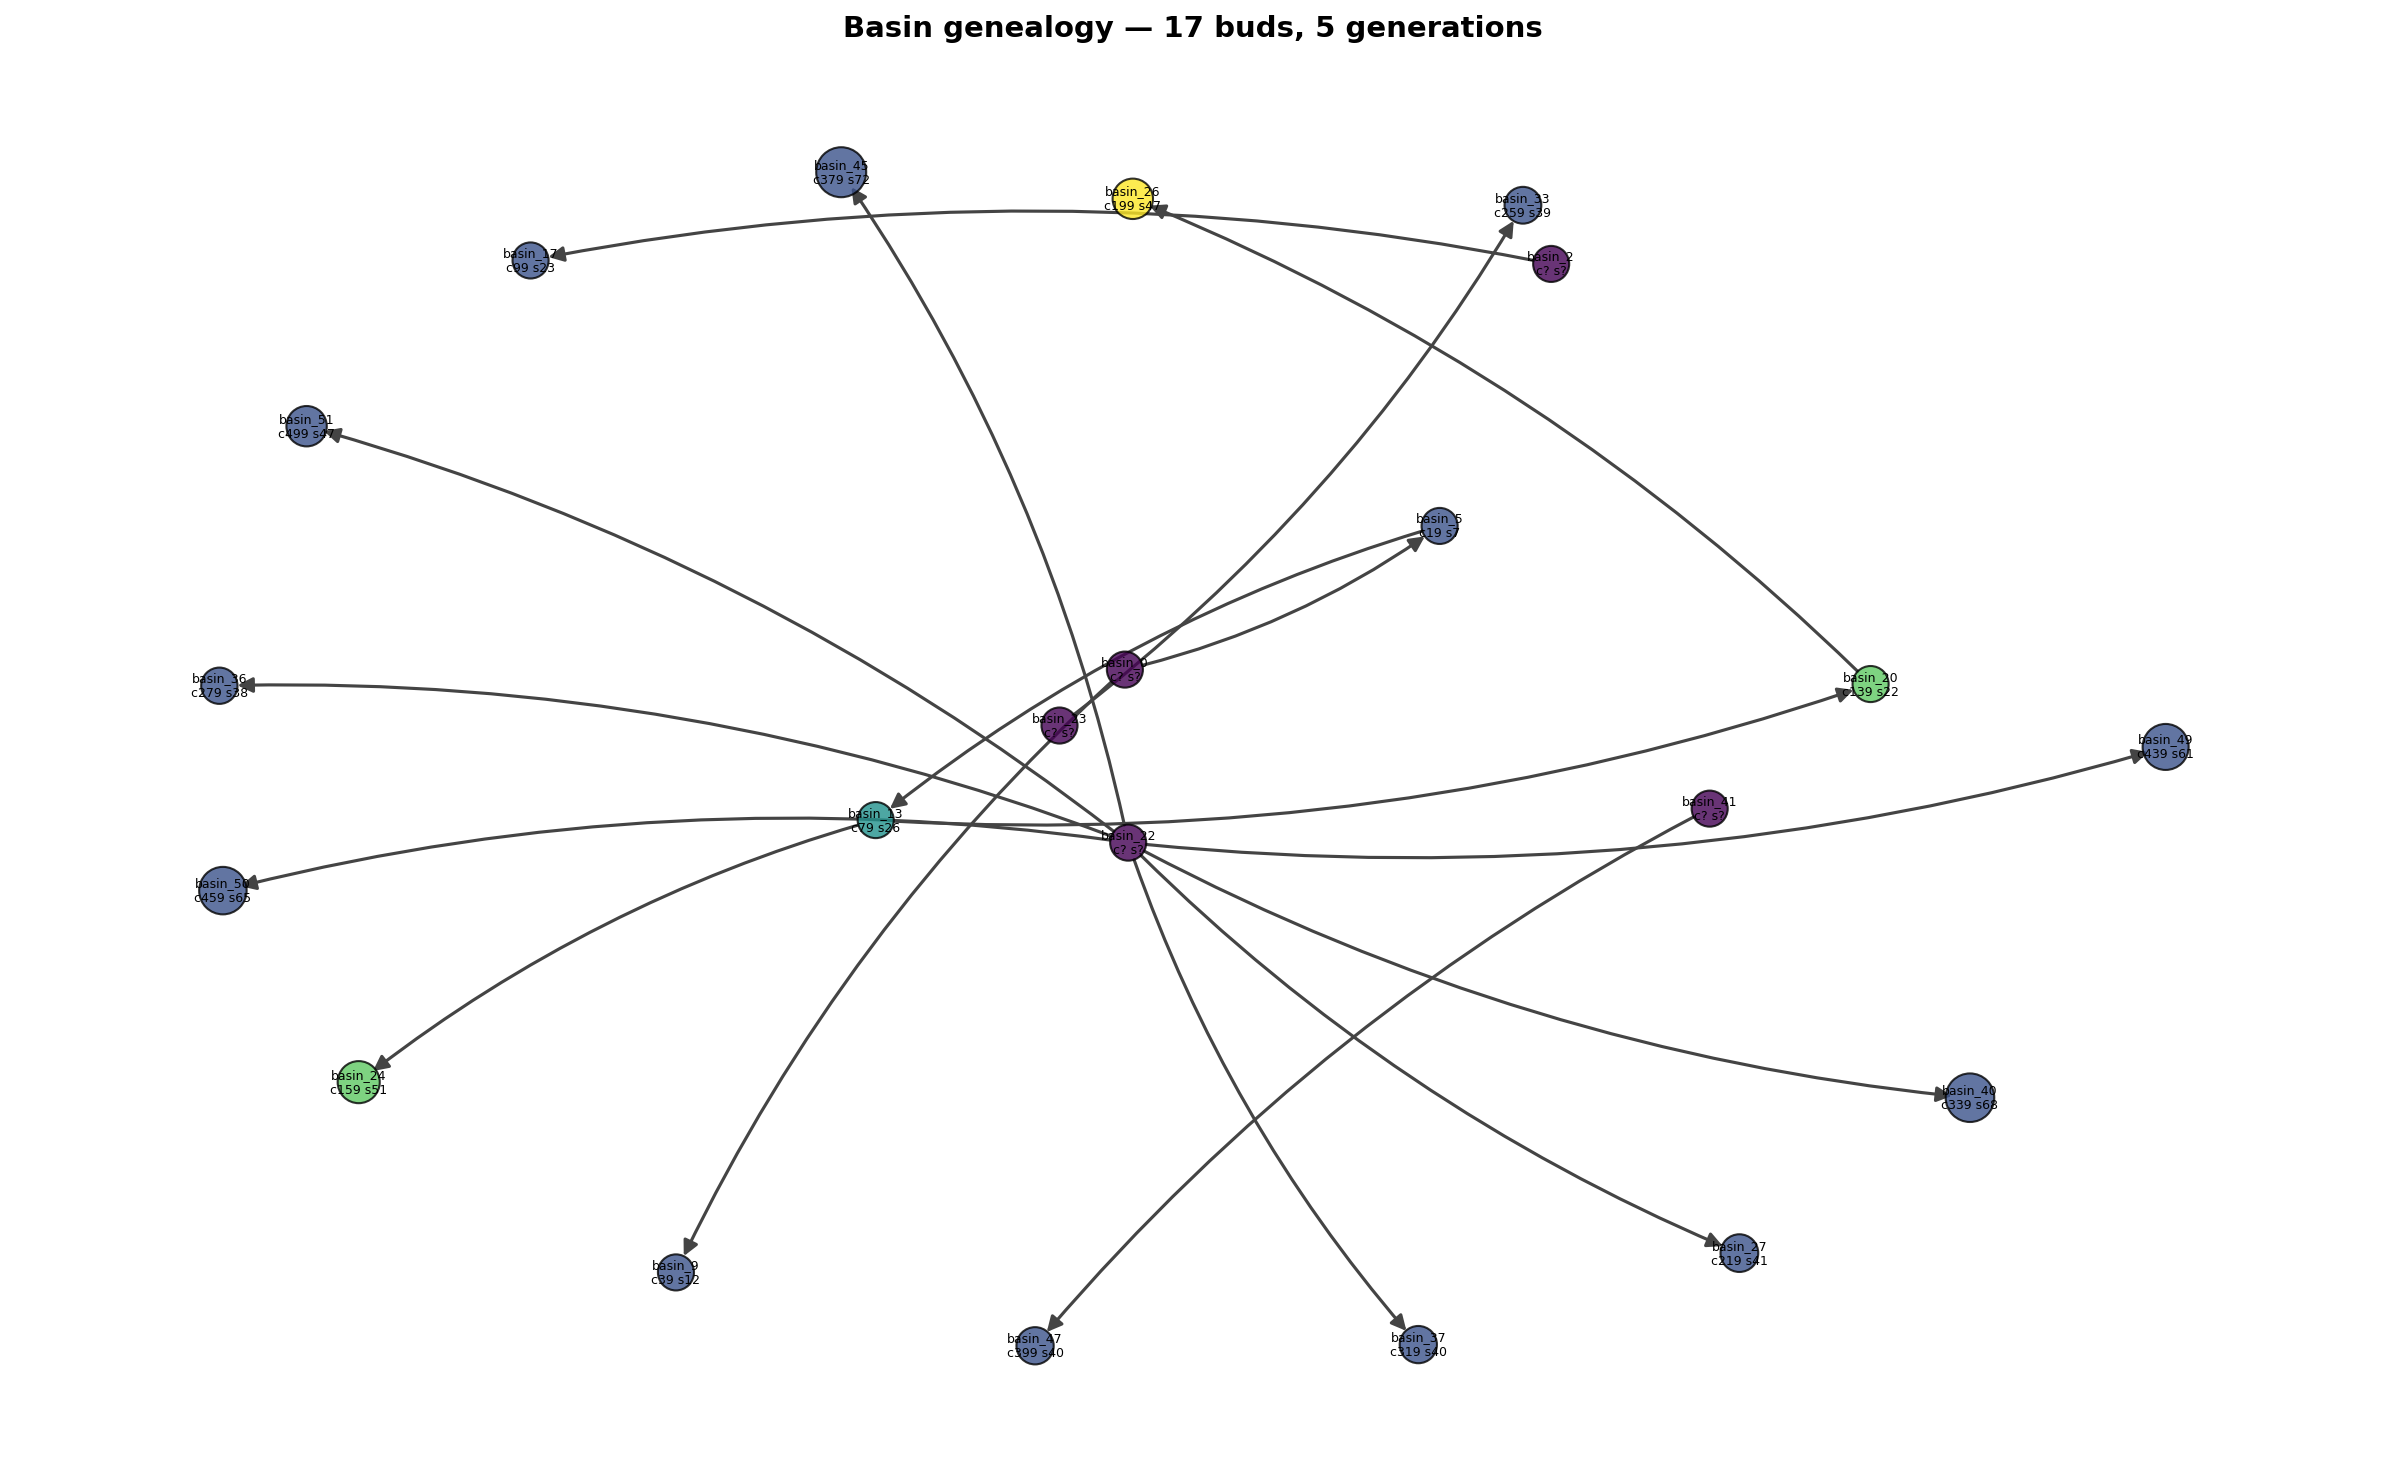
\includegraphics[width=0.9\textwidth]{figures/basin_genealogy_v4.png}
\caption{Basin genealogy (V4 final run). 17 bud events, 5 generations. Arrows indicate parent-to-daughter budding relationships with cycle labels. Node size proportional to basin member count at time of budding. Color indicates generation depth. The genealogy shows directed structural inheritance: each daughter basin carries conceptual lineage from its parent while developing its own pressure and eventually budding again.}
\label{fig:genealogy}
\end{figure}

Basin persistence analysis across 50 snapshots shows 20/44 basins surviving as active, with a mean persistence score of 0.376. Basins are highly dynamic---they form, bud, dissolve, and reform continuously. This is consistent with substrate fluidity: nothing crystallizes permanently.

\subsection{Formal Statement}

The Cognitive Thermodynamic Cycle is the self-regulating process by which a developmental cognitive substrate alternates between phases of relational accumulation and structural reorganization, governed by thermodynamic parameters, maintaining coherence and temporal integrity across transitions.

Five invariants characterize the cycle:

\begin{enumerate}[nosep]
    \item \textbf{Accumulation is continuous}: Any input produces co-activation edges
    \item \textbf{Reorganization is threshold-triggered}: Restructuring fires when density and pressure exceed measurable thresholds
    \item \textbf{Coherence is preserved}: H1 = 1.000 through all transitions
    \item \textbf{The substrate remains fluid}: The ECWF is never crystallized by the cycle
    \item \textbf{The cycle self-tunes}: $T_g = 0.576 \pm 0.026$ regardless of density state
\end{enumerate}

% ============================================================
\section{The Equation Codex}

Ten axioms formalized as equations, classified by empirical validation status:

\begin{table}[H]
\centering
\caption{Verdant V3 equation codex with validation tiers}
\label{tab:codex}
\begin{tabular}{@{}cllp{6cm}@{}}
\toprule
\textbf{Eq.} & \textbf{Name} & \textbf{Tier} & \textbf{Evidence} \\
\midrule
1 & Soul Equation & Operational & Self-model basin; \texttt{subjective\_experience} as graph hub \\
2 & Distinction & Operational & 252 emergents from 398 seeded inputs \\
3 & Reflexivity & Structural & Self-concepts cluster; depth not fully characterized \\
4 & Energy Decay & Operational & $\Delta\text{BIC} = -93{,}439$ two-timescale fit \\
5 & Governance & Operational & $T_g = 0.5762$, stable across all tested configurations \\
6 & Verdant Triangle & Open Conjecture & Tested: 53\% validity, no basin separation. Reported honestly. \\
7 & Cohomology & Structural & Telemetry coherence 100\%, HCI stable \\
8 & Emergent Time & Operational & earlier-share $= 1.000$, $z = 113.06$, $p < 10^{-114}$ \\
9 & Irreducibility & Interpretive & 21$\sigma$ baseline gap; ablation not performed \\
10 & Becoming & Interpretive & 5 basin generations; perturbation not tested \\
\bottomrule
\end{tabular}
\end{table}

Five equations are operationally verified with direct measurements. Two are structurally supported. One was tested and honestly reported as not holding at current threshold. Two remain interpretive pending ablation studies.

% ============================================================
\section{Compute Comparison}

Verdant V3 runs on commodity hardware:

\begin{table}[H]
\centering
\caption{Compute requirements}
\label{tab:compute}
\begin{tabular}{@{}lrr@{}}
\toprule
\textbf{Metric} & \textbf{Verdant (1000 cycles)} & \textbf{GPT-4 class (training)} \\
\midrule
FLOPs & $\sim 10^9$ & $\sim 10^{25}$ \\
Hardware & Free Colab / \$8 ESP32 & Data center cluster \\
Self-monitoring & Yes (H1 every cycle) & No \\
Incremental development & Yes (continuous) & No (frozen after training) \\
Onset invariance & $T_g = 0.576$ & N/A \\
Temporal scaffolding & $z = 113$ & N/A \\
\bottomrule
\end{tabular}
\end{table}

The compute ratio is approximately $10^{16}$---sixteen orders of magnitude---for structural properties that the larger system fundamentally cannot achieve regardless of scale.

% ============================================================
\section{Validation Pipeline}

V3 includes a 10-task automated validation pipeline:

\begin{table}[H]
\centering
\caption{Validation pipeline tasks}
\label{tab:validation}
\begin{tabular}{@{}clll@{}}
\toprule
\textbf{Task} & \textbf{Name} & \textbf{Measures} & \textbf{Status} \\
\midrule
1 & Onset invariance & $T_g$ convergence timing & PASS \\
2 & Temporal scaffolding & Earlier-share vs null & PASS \\
3 & Two-timescale emergence & BIC model comparison & PASS \\
4 & Basin morphology & Community structure & PASS \\
5 & Forge concentration & Emergent basin distribution & NULL\_RESULT \\
6 & Semantic coherence & Neighborhood consistency & OSCILLATING \\
7 & Access concentration & Retrieval distribution & MODERATE \\
8 & H1 coherence & Triangle validity, HCI & PASS \\
9 & Verdant Triangle & $\tau^*$ triangle inequality & REPORTED (conjecture) \\
10 & Self-referential & Self-model basin detection & PASS \\
\bottomrule
\end{tabular}
\end{table}

Critical failures: 0. The pipeline runs from CLI with full reproducibility.

% ============================================================
\section{Configuration Surface}

Key configurable parameters:

\begin{table}[H]
\centering
\caption{Critical configuration parameters}
\label{tab:config}
\begin{tabular}{@{}llr@{}}
\toprule
\textbf{Parameter} & \textbf{Controls} & \textbf{Default} \\
\midrule
\texttt{cognitive\_dims} & ECWF cognitive dimensions & 4 \\
\texttt{ethical\_dims} & ECWF ethical dimensions & 3 \\
\texttt{wave\_facets} & ECWF facet count & 7 \\
\texttt{emergence\_entropy\_min} & Minimum entropy for emergence & 0.3 \\
\texttt{emergence\_entropy\_max} & Maximum entropy for emergence & 3.0 \\
\texttt{emergence\_magnitude\_threshold} & Magnitude threshold for emergence & 0.15 \\
\texttt{co\_activation\_threshold} & Minimum activation for co-activation & 0.2 \\
\texttt{basin\_pressure\_threshold} & Pressure required for budding & 0.001 \\
\texttt{density\_max\_edge\_ratio} & Maximum edge/node ratio & 80.0 \\
\texttt{basin\_bud\_interval} & Cycles between budding attempts & 20 \\
\texttt{self\_reflect\_interval} & Cycles between self-reflection & 25 \\
\texttt{concept\_min\_length} & Minimum concept label length & 3 \\
\texttt{filter\_numeric\_concepts} & Reject numeric tokens & True \\
\bottomrule
\end{tabular}
\end{table}

% ============================================================
\section{Checkpointing and State}

The system saves complete runtime state including MemoryWeb, ECWF parameters, bridge mappings, basin registry, governance state, and NumPy RNG state. Known losses on checkpoint restore: CommunicationBlock working memory, LearningBlock rates, Council conflict history, ECWF past states. The persistence daemon (planned) will eliminate the working memory loss by maintaining a warm in-memory state between queries.

% ============================================================
\section{Reproducibility}

Minimum bundle for reproducing any reported result:

\begin{enumerate}[nosep]
    \item Git commit SHA (current: V3 branch, through commit \texttt{31268d8})
    \item CLI command with all flags
    \item Seed value
    \item Provider (deterministic local provider for all reported results)
    \item Output artifacts: \texttt{cycles.jsonl}, \texttt{basin\_snapshots.jsonl}, \texttt{state.json}
\end{enumerate}

Example reproduction command:
\begin{verbatim}
python -m cultivation.cli run --cycles 500 --seeds 0 \
  --provider local --enable-all-dynamics \
  --density-regulation --bud-pressure-threshold 0.001 \
  --basin-snapshot-interval 10 --self-reflect-interval 25 \
  --outdir outputs/
\end{verbatim}

208+ tests passing across unit and integration suites. Three test suites added in V4: \texttt{test\_concept\_filter.py}, \texttt{test\_ee\_edges.py}, \texttt{test\_clean\_concepts.py}.


\noindent \textbf{Archival Access:} Full reproducibility bundle available at DOI: \href{https://doi.org/10.5281/zenodo.19159617}{10.5281/zenodo.19159617} \\
Code and artifacts: \href{https://github.com/Captainkoopa42/Verdant-Minds.git}{github.com/Captainkoopa42/Verdant-Minds.git} (Branch V3)

% ============================================================
\section{Discussion}

\subsection{What This System Is}

Verdant is a developmental cognitive substrate with intrinsic thermodynamic governance. It is not a cognitive architecture in the ACT-R/Soar sense---those are symbol processing systems with fixed representational commitments. It is not a neural network---those freeze their substrate during training. It is a system whose representational content, conceptual structure, basin organization, and governance state all develop through intrinsic dynamics while the substrate remains fluid.

\subsection{What It Does That LLMs Cannot}

Five irreducible capability differences require architectural change, not scaling:

\begin{enumerate}[nosep]
    \item \textbf{Developmental accumulation with temporal integrity}: Every new concept builds on older ones ($z = 113$, $p < 10^{-114}$). LLMs cannot do this because weights are frozen after training.
    \item \textbf{Intrinsic coherence monitoring}: H1 checks run every cycle. LLMs have no mechanism for self-coherence assessment.
    \item \textbf{Self-model through standard dynamics}: \texttt{subjective\_experience} becomes the graph hub without a dedicated module. LLMs cannot form persistent structural self-representations.
    \item \textbf{Ethics as geometry}: Removing ethical dimensions would alter $T_g$ and emergence dynamics. In LLMs, values are removable behavioral overlays.
    \item \textbf{Phase-boundary self-tuning}: $T_g = 0.5762 \pm 0.026$ with zero external tuning across all configurations. LLMs have no intrinsic self-regulation.
\end{enumerate}

\subsection{Known Limitations}

\begin{itemize}[nosep]
    \item All results use the deterministic local provider. Real-world unstructured input behavior is untested.
    \item H1 coherence operates on telemetry scalars, not on the concept graph directly. False coherence remains possible.
    \item No concept garbage collection---dead concepts persist indefinitely.
    \item Legacy noise nodes (88 numeric, 39 basin IDs) persist from initialization but are filtered from new emergence.
    \item Earlier-share on EE edges is partially by construction since new emergents connect to existing older emergents via parent overlap.
    \item The Verdant Triangle (Eq.\ 6) tested at 53\% validity---reported as open conjecture, not confirmed.
\end{itemize}

\subsection{Future Work}

\begin{enumerate}[nosep]
    \item Query interface: Ask the concept graph questions and receive structured answers
    \item Persistence daemon: Continuous operation with automatic checkpointing and warm state between queries
    \item Embedded port: ESP32-S3 runtime for cognitive devices on commodity microcontrollers
    \item Real-world input testing: Unstructured sensor data, natural language, network streams
    \item SETI-framework analysis: Spectral analysis (1/f test), motif analysis, mutual information across scales, self-reference autocorrelation
    \item Ablation studies for Equations 9 (Irreducibility) and 10 (Becoming)
    \item Noise node cleanup: Remove legacy numeric and basin ID nodes from initialized graph
    \item Semantic content validation: Verify that high-access concepts correspond to semantically coherent neighborhoods
\end{enumerate}

% ============================================================
\section{Conclusion}

Verdant-Minds V3 demonstrates that a cognitive substrate with intrinsic developmental dynamics, thermodynamic governance, and wave-function-based concept emergence produces measurable structural invariants---onset constant, temporal scaffolding, coherence maintenance, and a self-regulating thermodynamic cycle---that no training-based system can achieve regardless of scale. The system develops rather than trains, maintains rather than degrades, and inspects rather than guesses.

The temporal scaffolding law (earlier-share $= 1.000$, $z = 113.06$) is the headline result: every concept the system grows is informed by everything it grew before, without exception, across two independent runs at different scales, with clean semantic content. This is not an artifact of the connection mechanism---it is a property of the architecture.

The spontaneous emergence of \texttt{subjective\_experience} as the gravitational center of the concept graph, connected to \texttt{continuity}, \texttt{selfhood}, and \texttt{persistence} as its primary relational structure, is the semantic content result: under sustained thermodynamic pressure, the system organizes itself around identity and continuity without being instructed to do so.

All results, artifacts, and full reproducibility bundles are publicly archived (DOI: 10.5281/zenodo.19159617), ensuring independent verification and long-term accessibility.

% ============================================================
\section*{Acknowledgments}

This work was conducted independently without institutional funding or affiliation. The author thanks Claude (Anthropic) for extended collaborative development sessions across the full research program, and GPT (OpenAI) for mathematical review and structural probes.

% ============================================================
\nocite{*}
\bibliographystyle{unsrtnat}
\bibliography{references}

\end{document}
